\Exhibit{ChelyabinskTv}{
    Скриншоты и транскрипт дискуссии об инженерах на областном телевидении Челябинской области,
    показывающие продукты Школы Граня\WithTr%
}

Это скриншоты и транскрипт инженерной дискуссии.
Эта программа вышла 1 марта 2023 на канале `Первое областное информагентство'
Челябинской области.

Достоверность видео подтверждается тем, что оно на сайте `1obl.ru', принадлежащем каналу.

В этом видео показаны обучающие наборы, производимые Школой Граня,
и логотип школы чётко виден на двух из них.

\begin{itemize}
    \item На 02:13 показан набор с тепловым двигателем.
    \item На 02:43 показан набор для работы с глиной.
\end{itemize}

Высокоранговость дискуссии подтверждается участием
Виталия Литке, Заместителя министра оборазования и науки Челябинской области
показанного на 30:32.

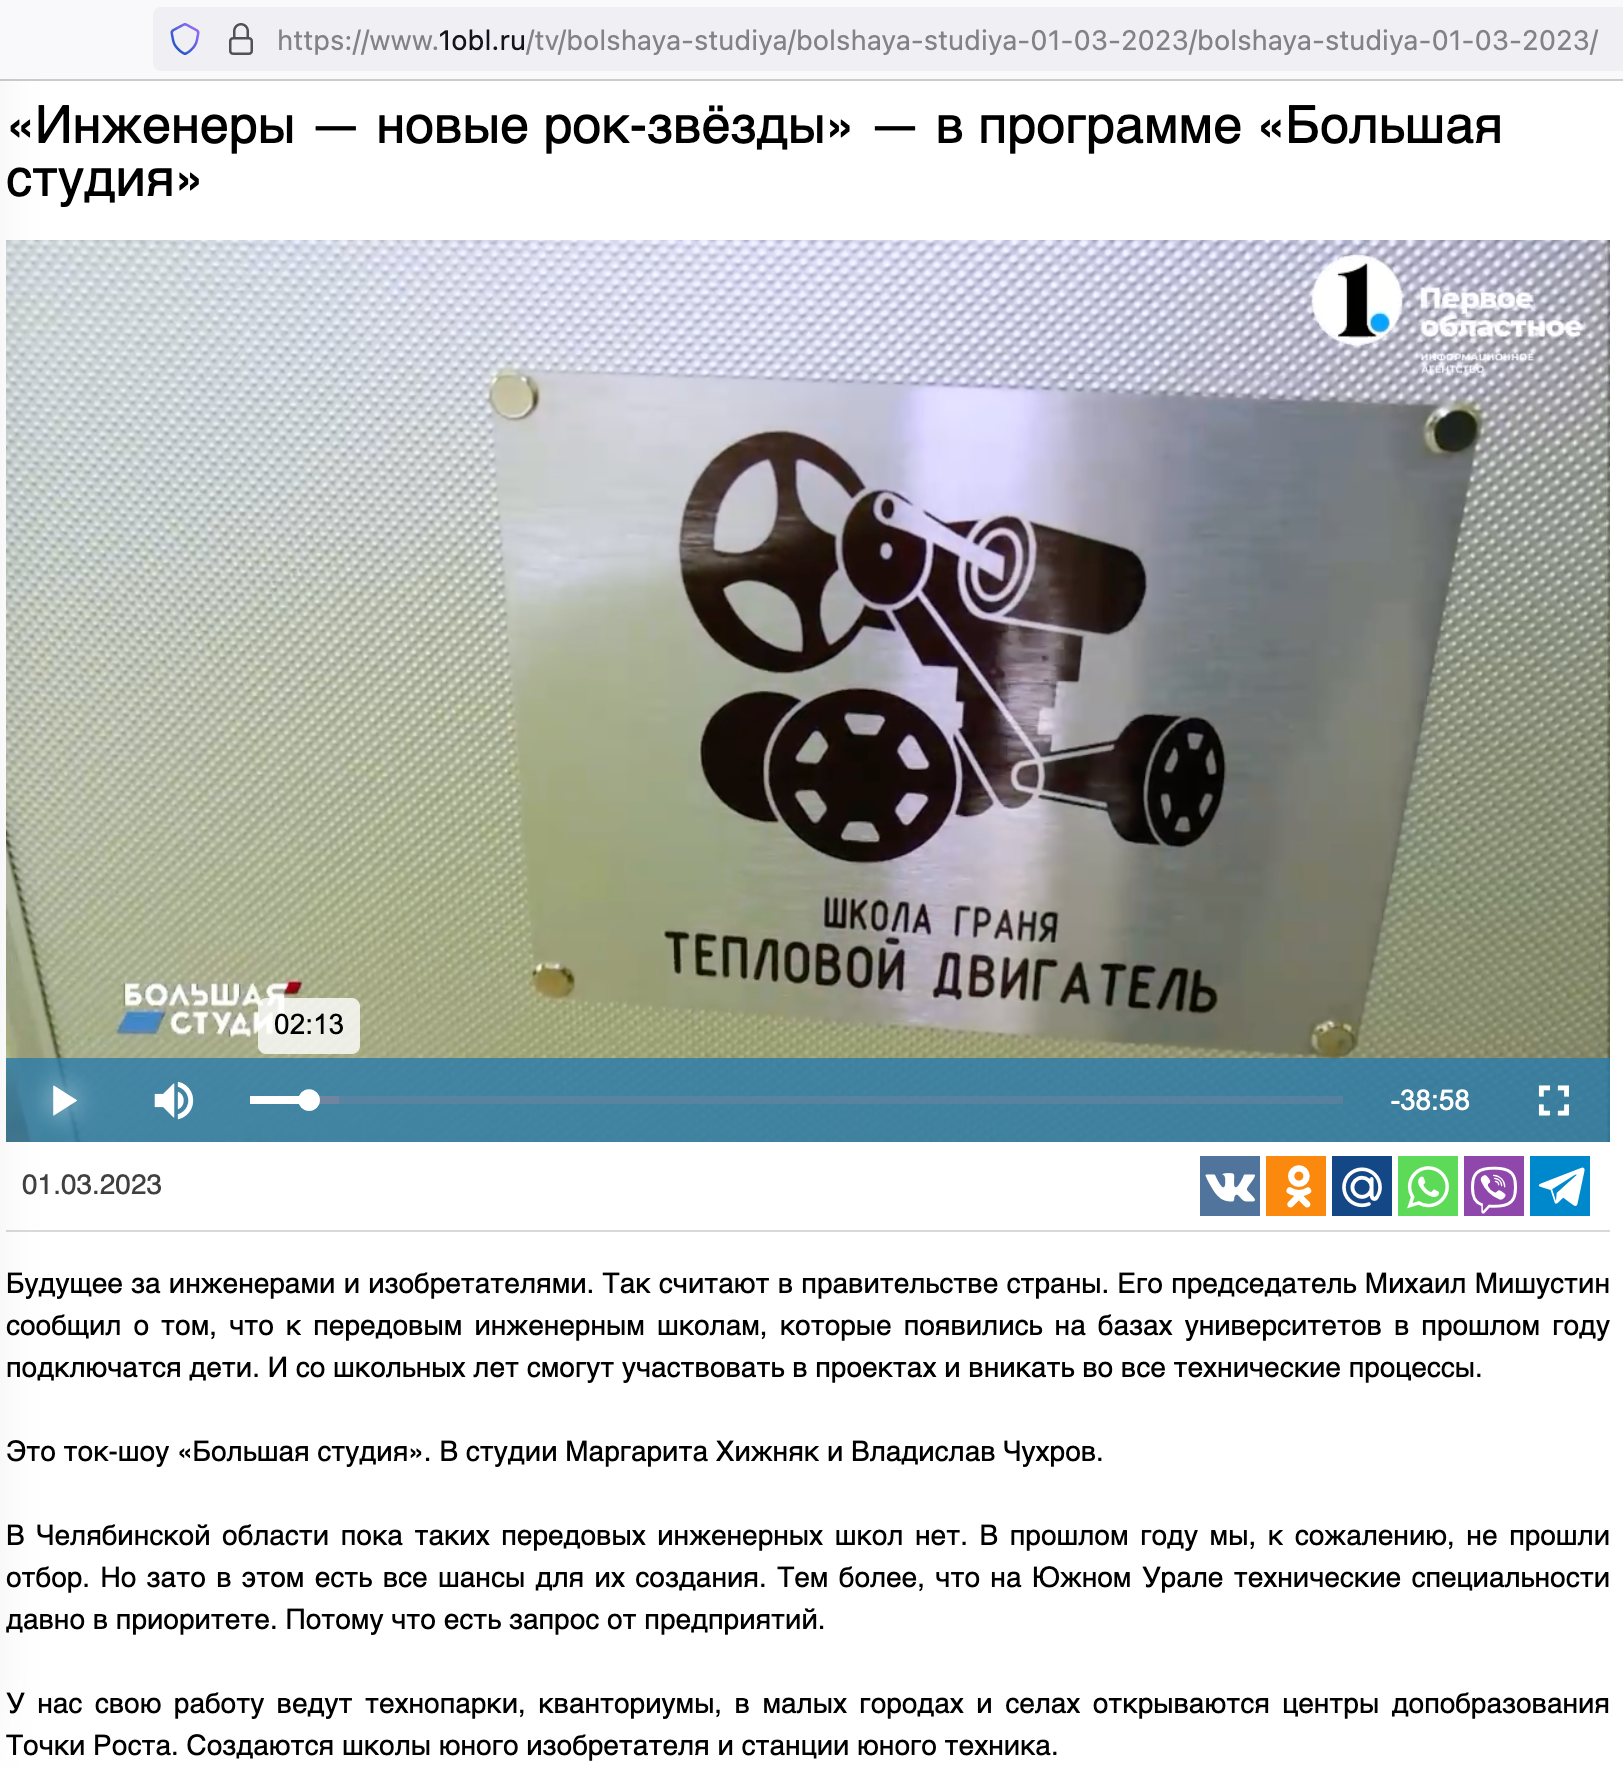
\includegraphics[width=\textwidth]{bag}
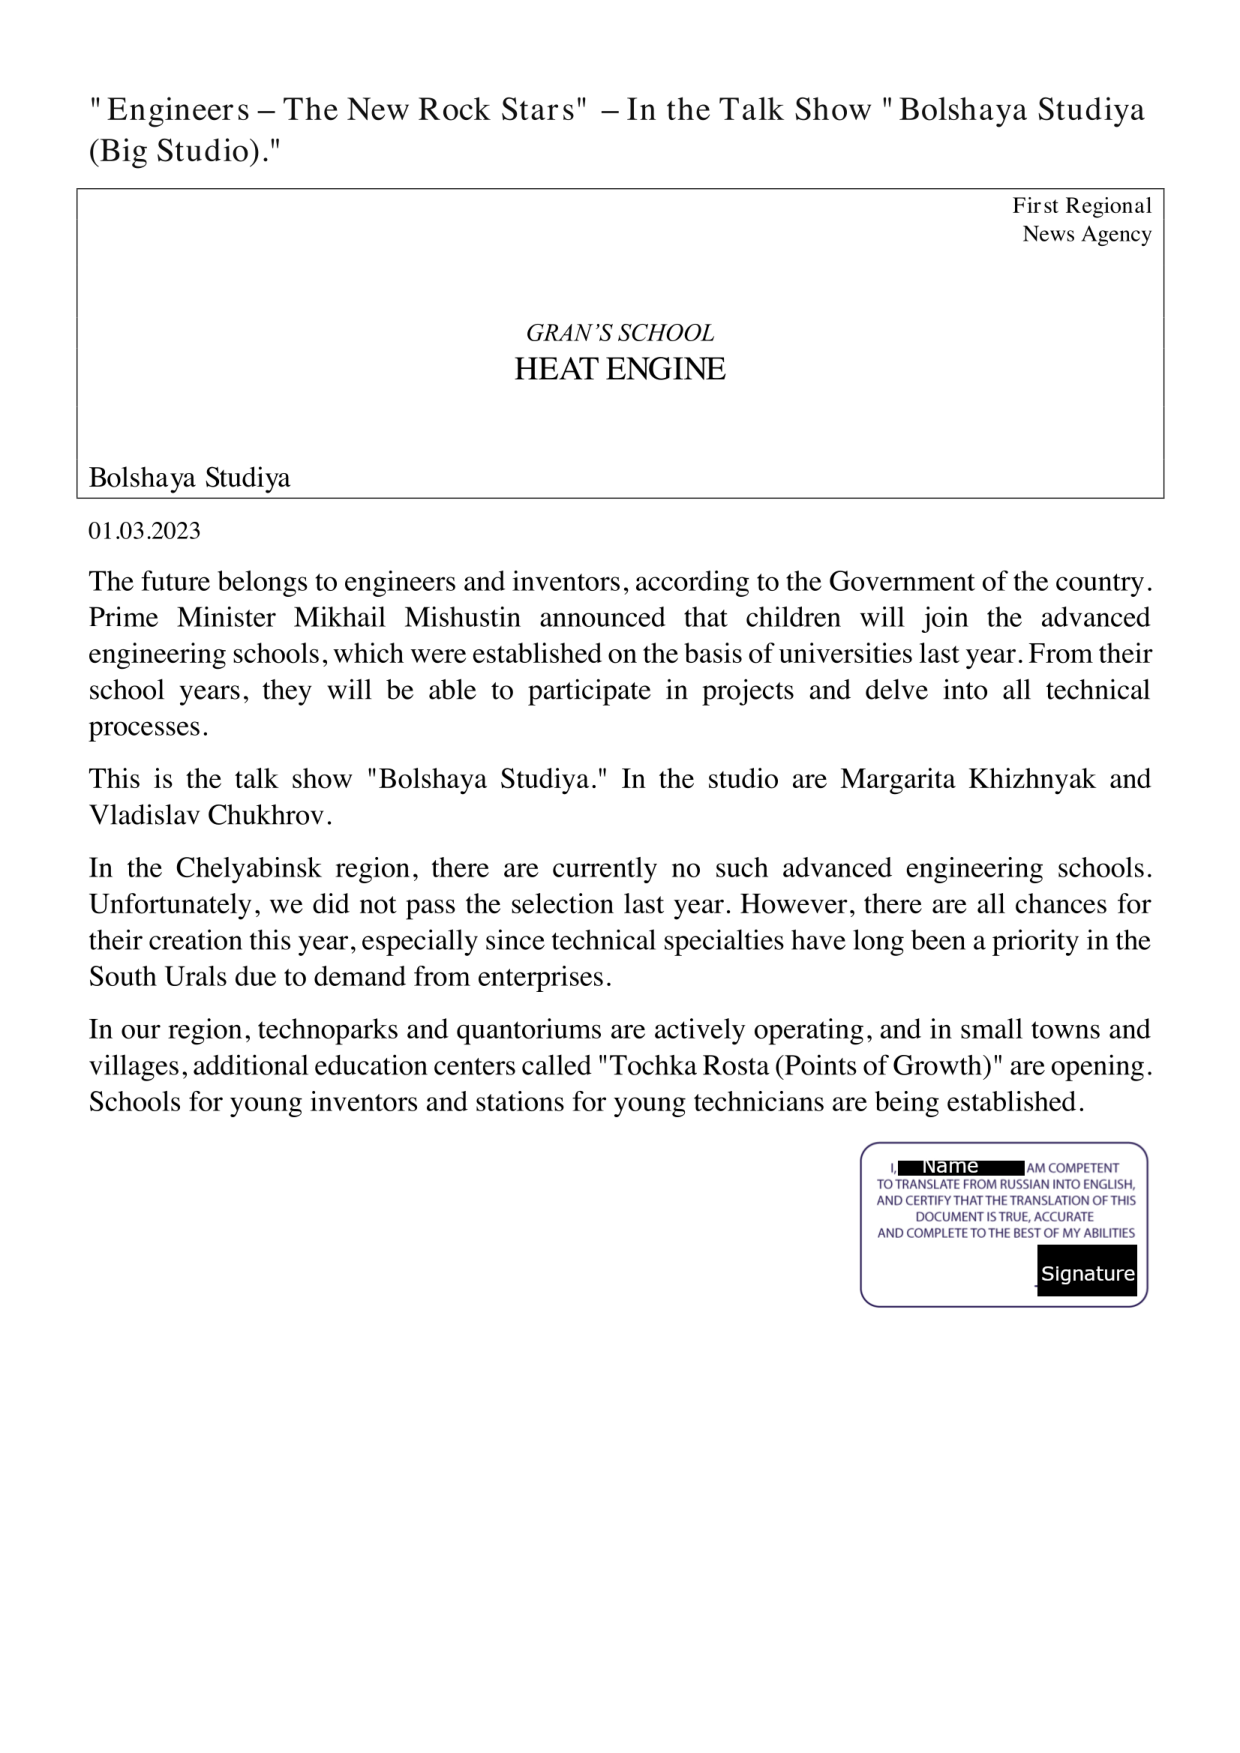
\includepdf[pages=-]{bag_eng_public}

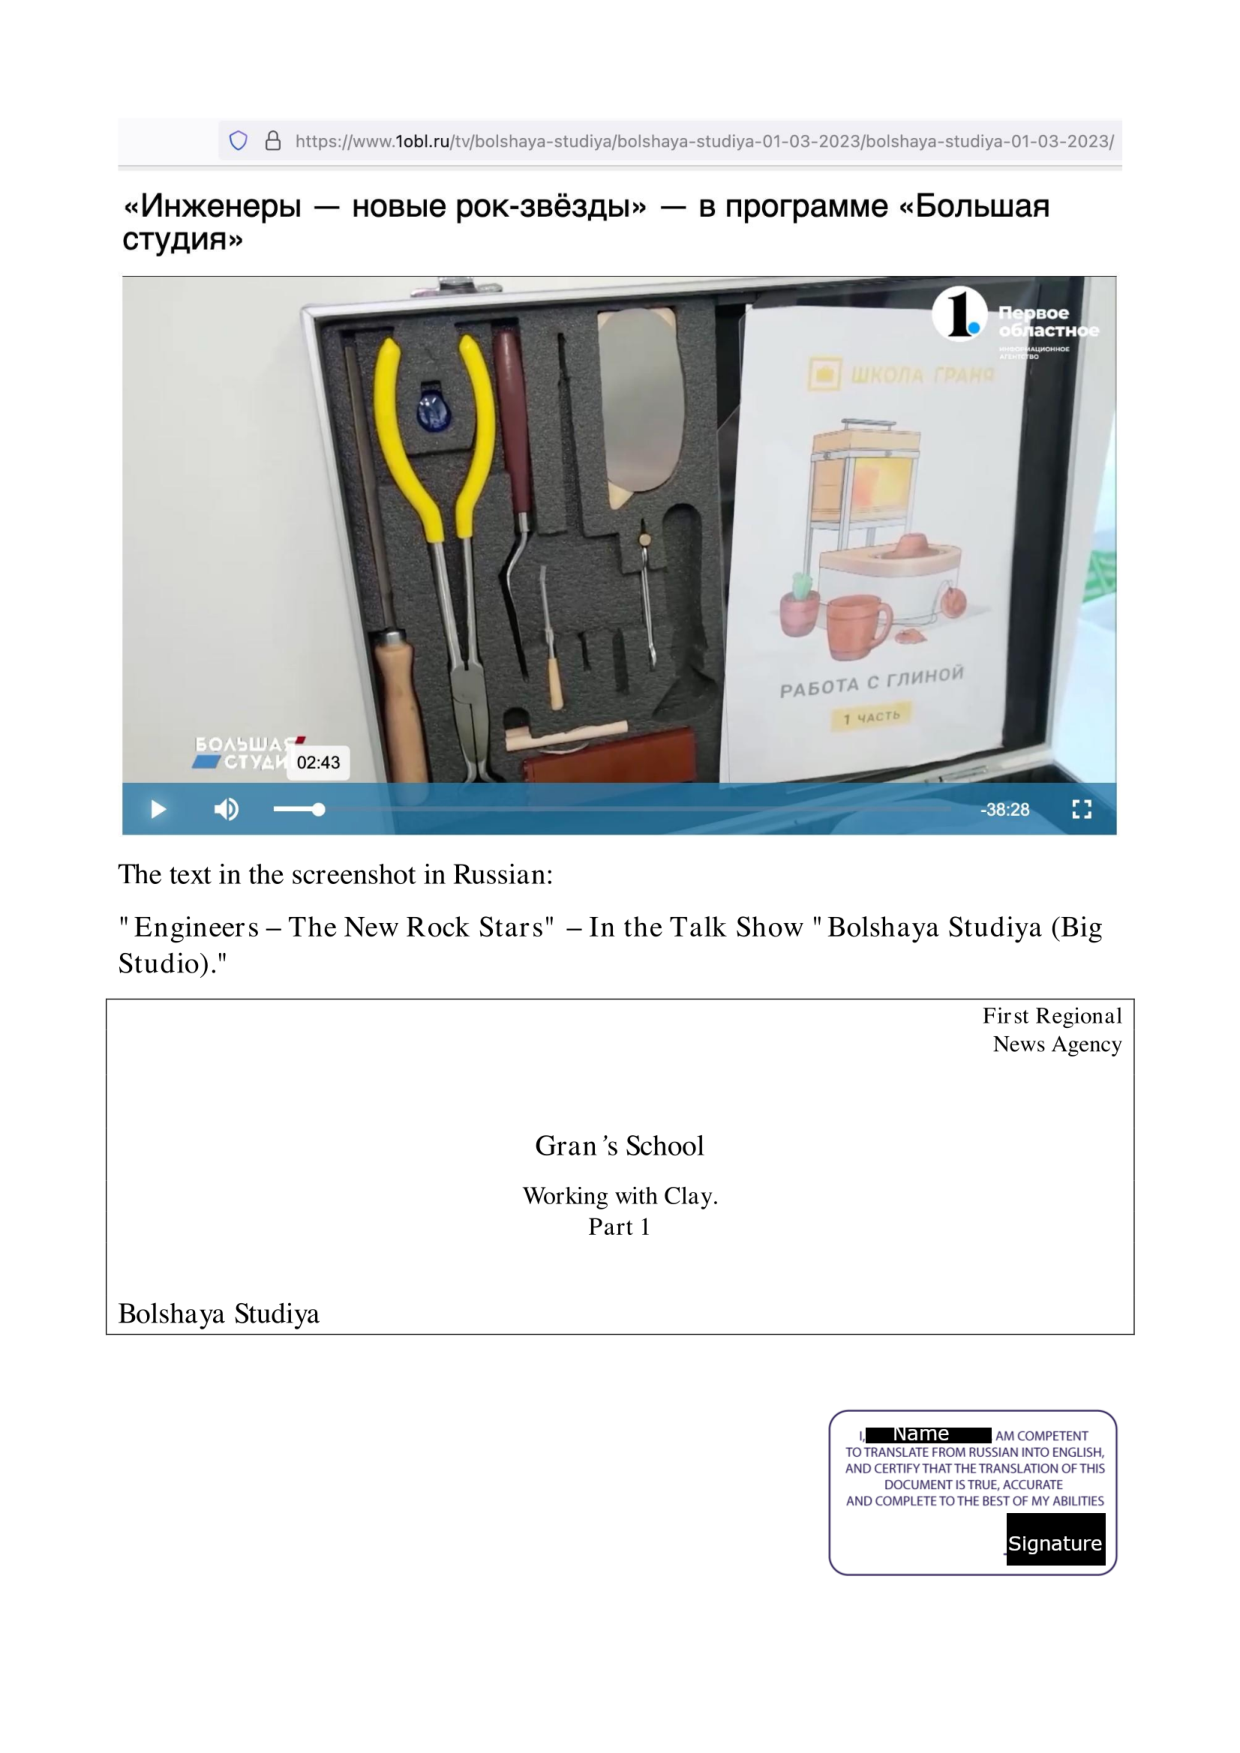
\includepdf[pages=-]{clay_eng_public}

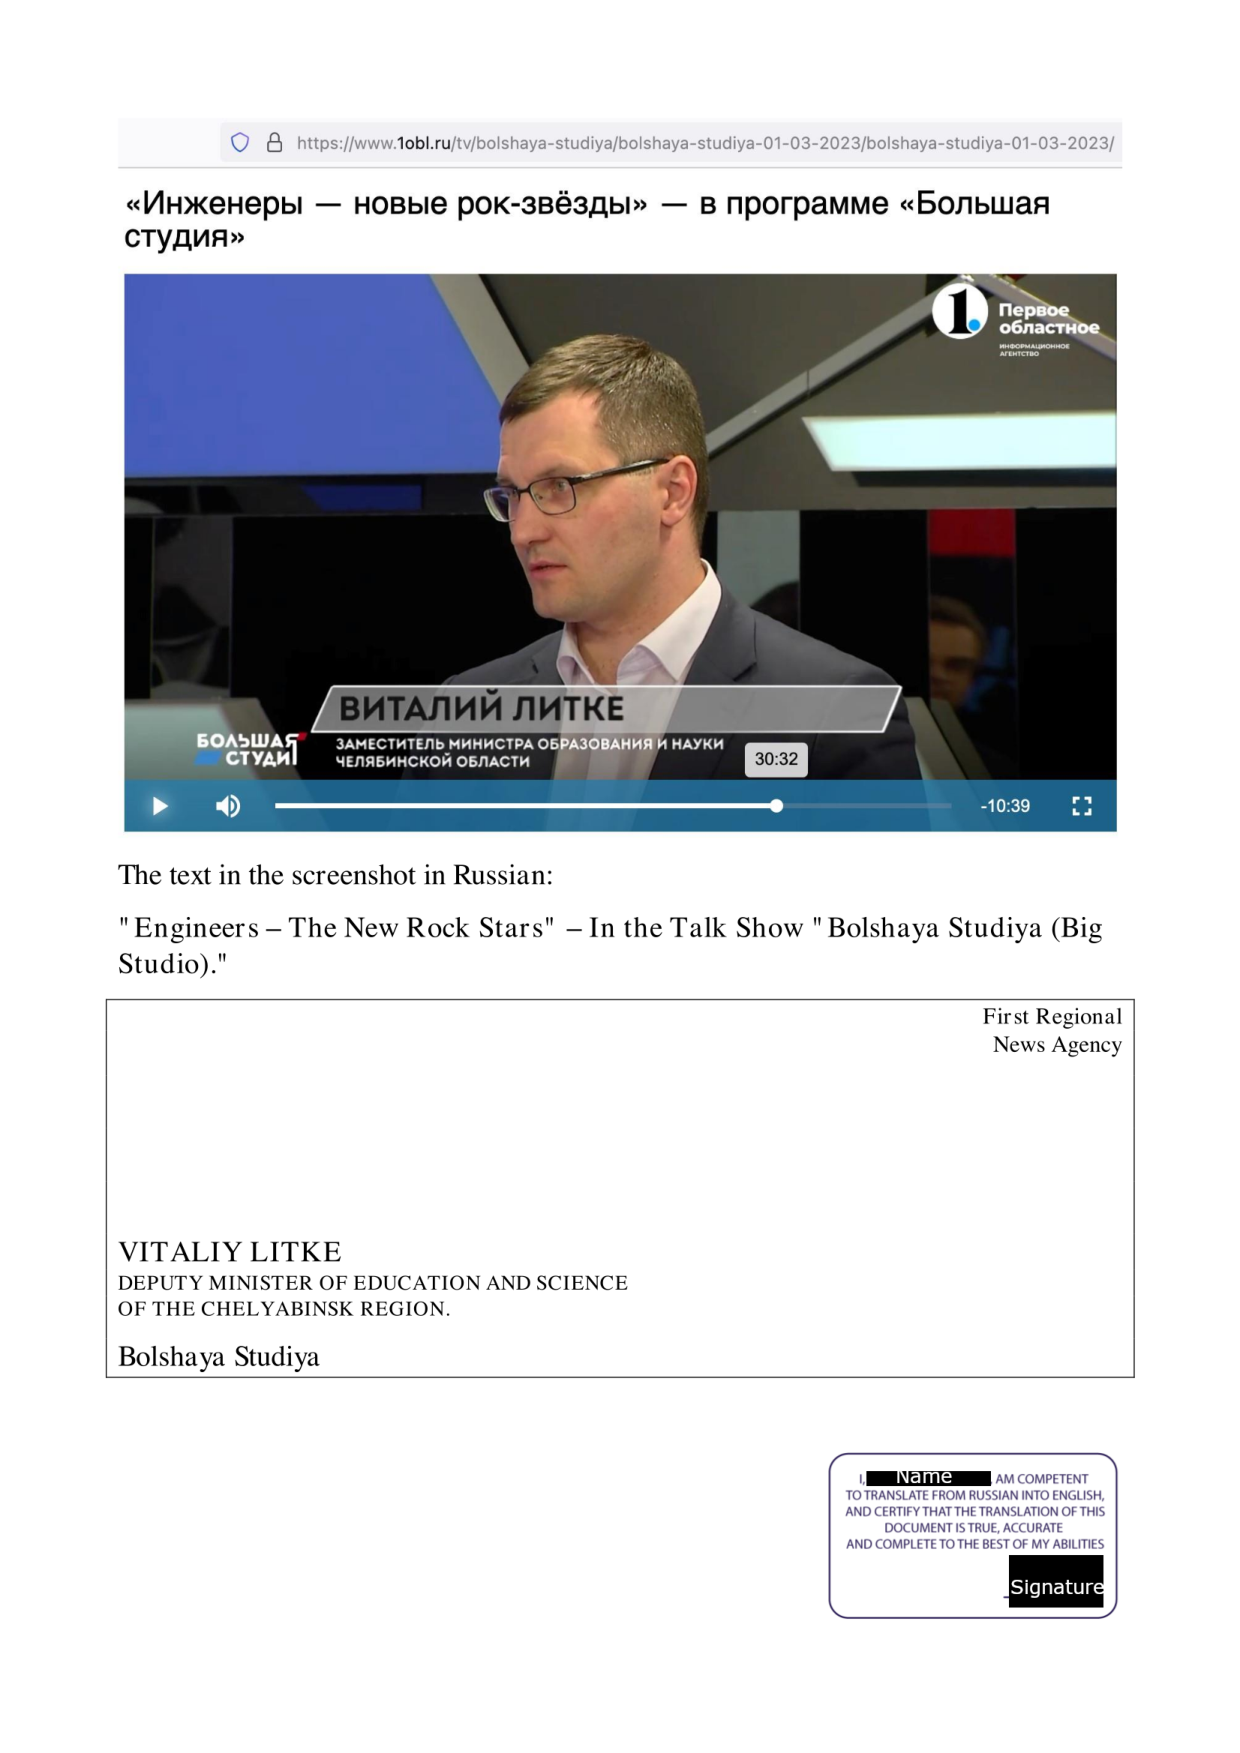
\includepdf[pages=-]{minister_eng_public}

Демонстрация наборов Школы Граня и рассказ о них идёт с
02:12 до 07:22 -- 5 минут и 10 секунд экранного времени,
см. транскрипт:

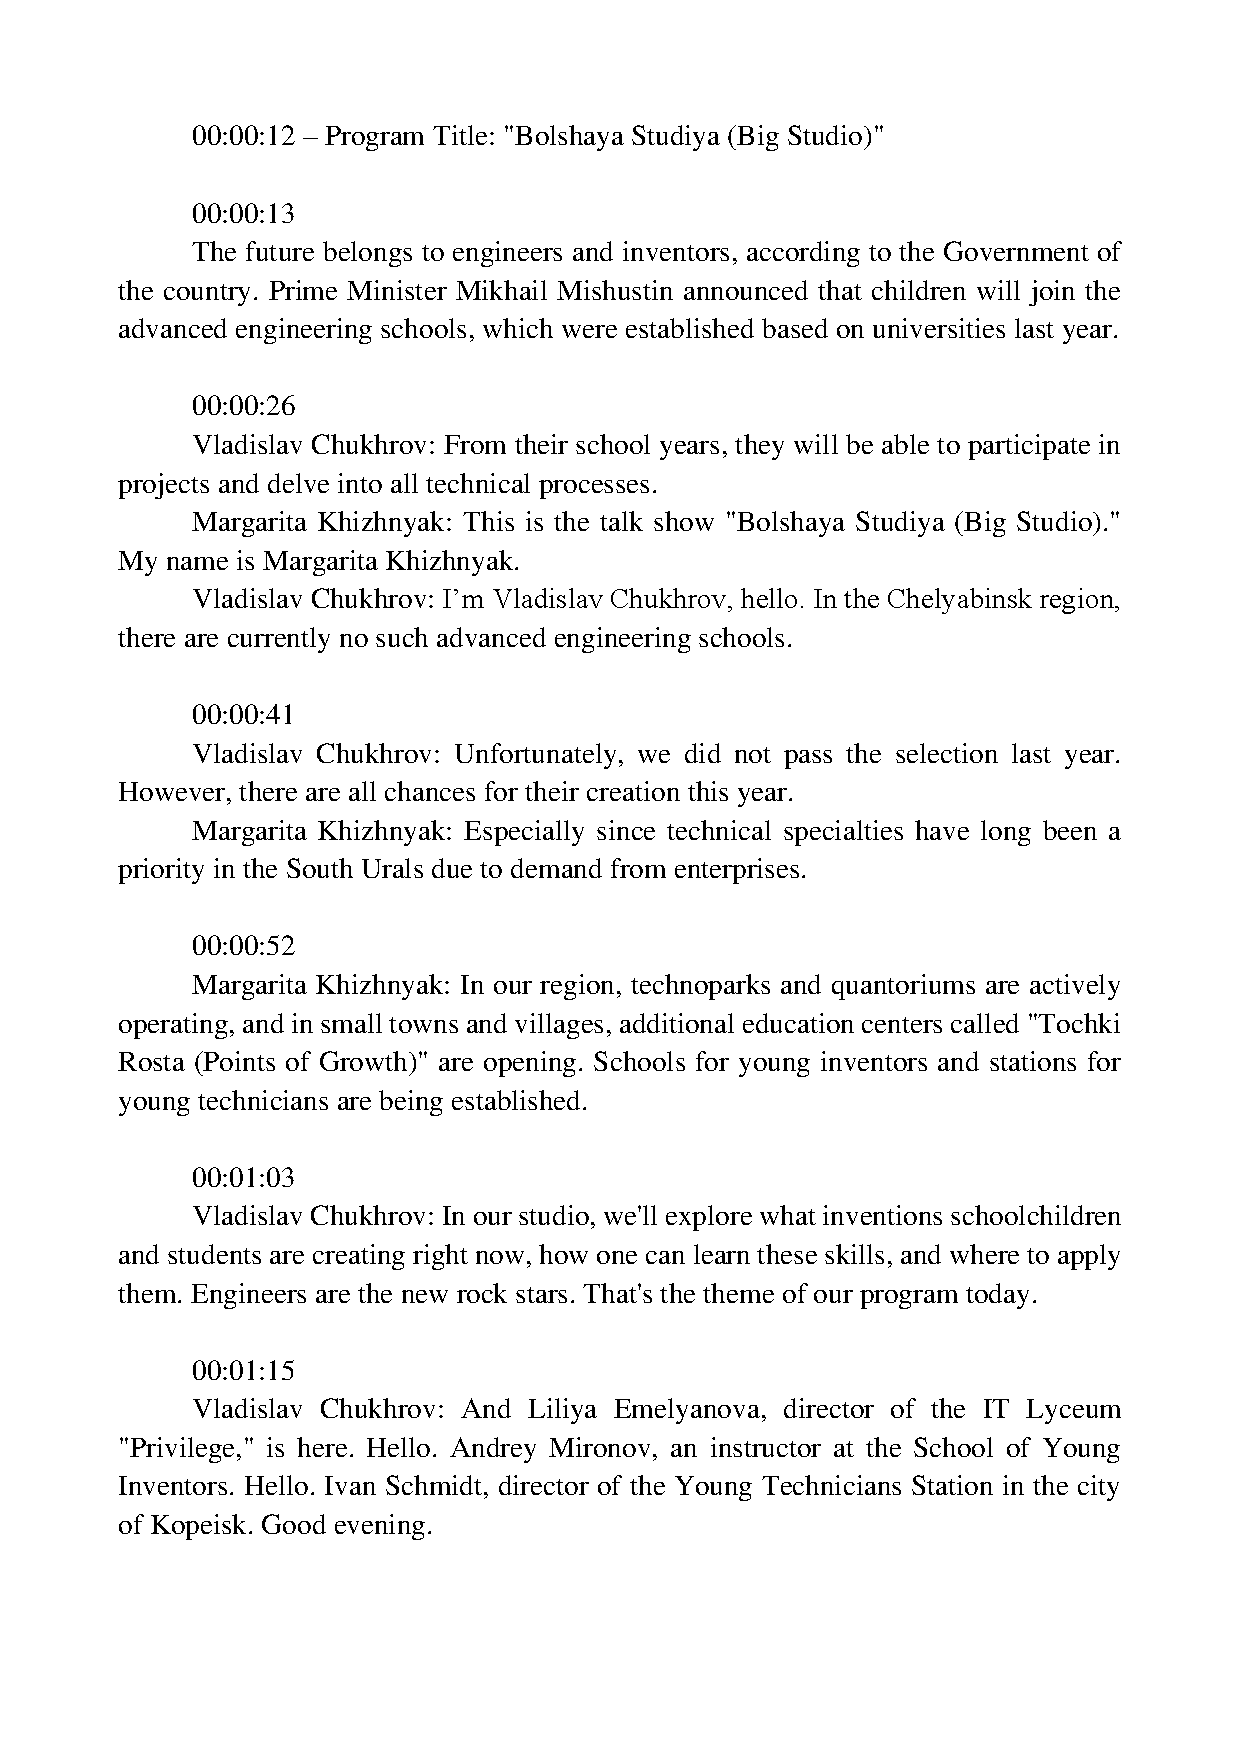
\includepdf[pages=-]{transcript_to-7-22_eng_public}

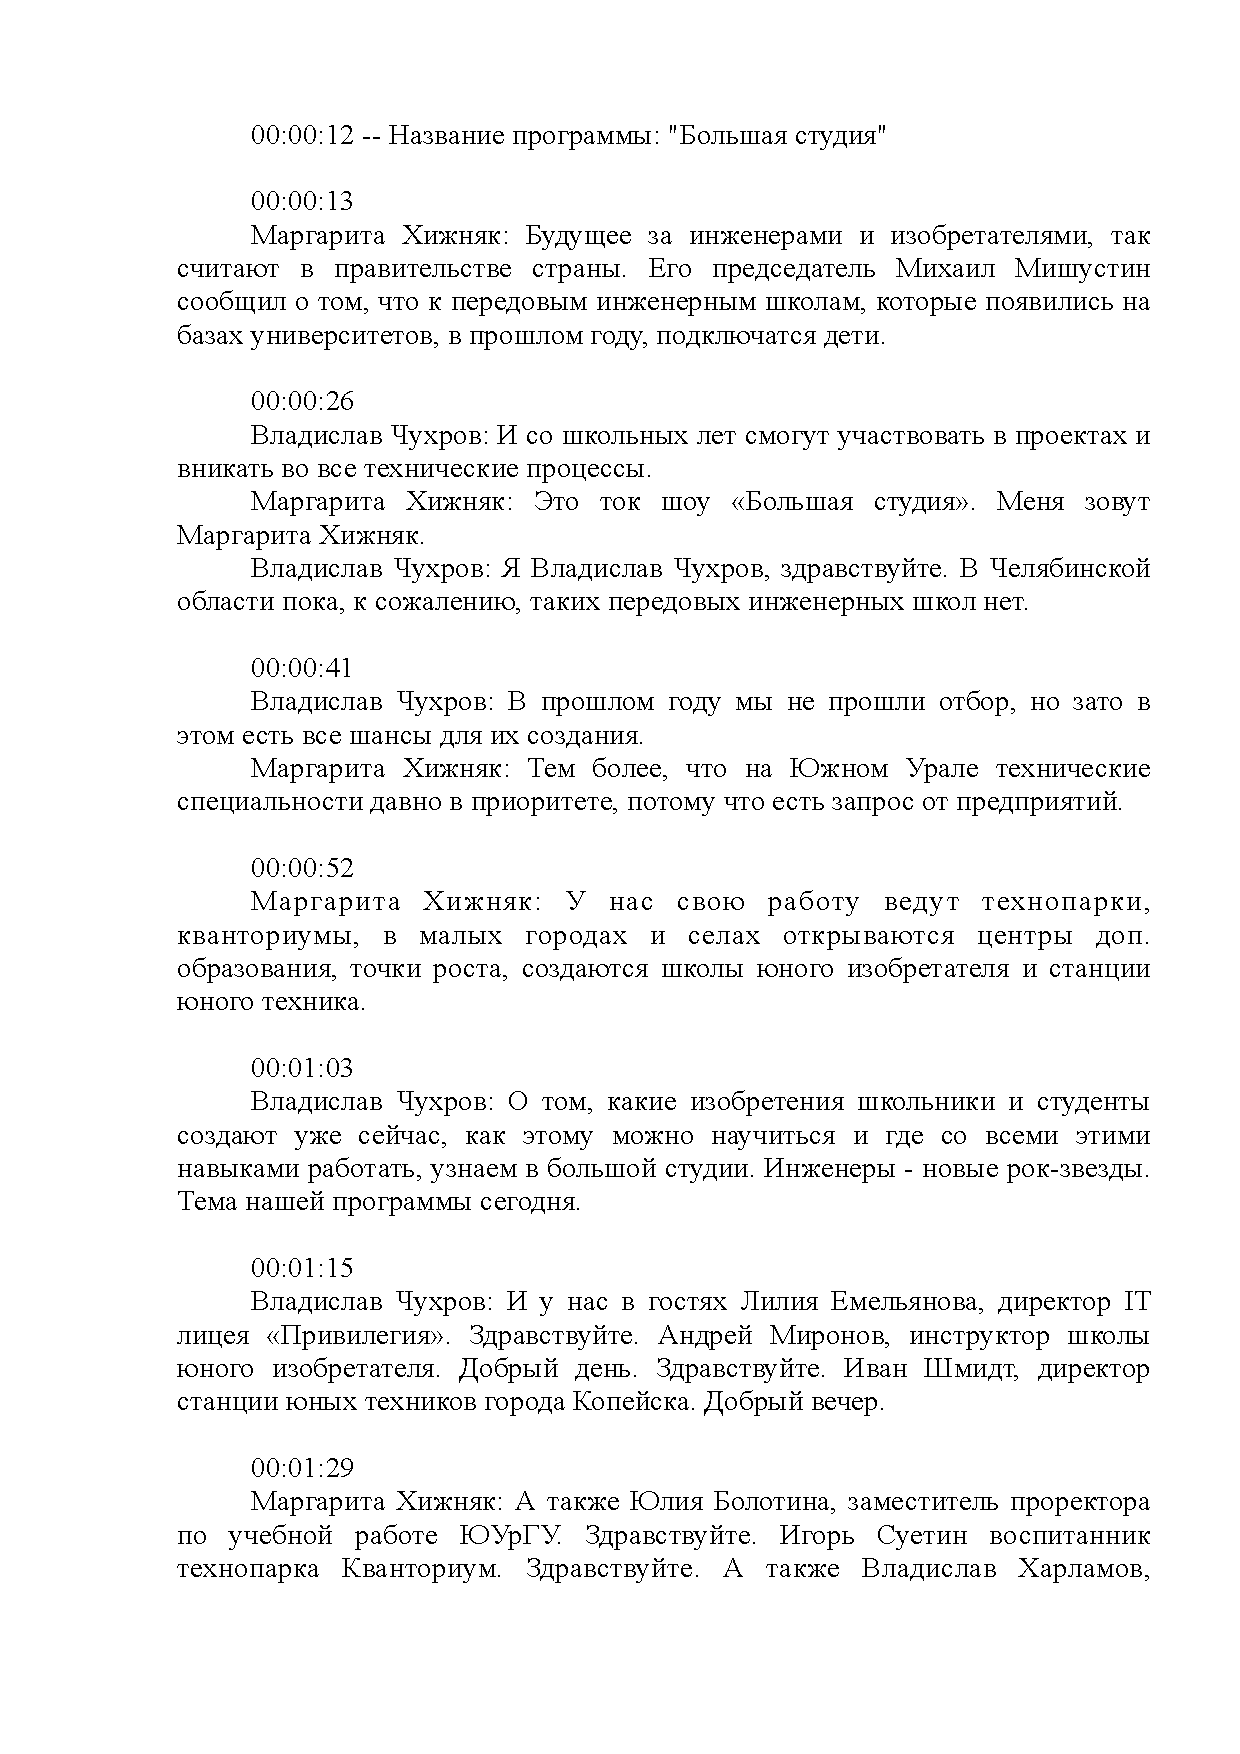
\includepdf[pages=-]{transcript_to-7-22}

\pagebreak
